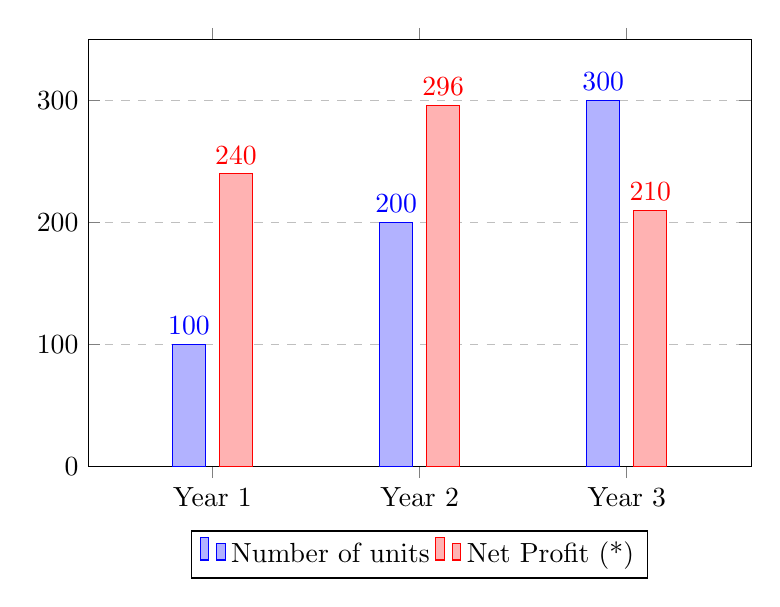
\begin{tikzpicture}
\begin{axis}[
    ybar=5pt,
    bar width=12pt,
    width=10cm, height=7cm,
    ymin=0, ymax=350,
    ylabel={},
    symbolic x coords={Year 1, Year 2, Year 3},
    xtick=data,
    nodes near coords,
    legend style={at={(0.5,-0.15)},anchor=north,legend columns=-1},
    enlarge x limits=0.3,
    ymajorgrids=true,
    grid style=dashed
]
\addplot coordinates {(Year 1, 100) (Year 2, 200) (Year 3, 300)};
\addplot coordinates {(Year 1, 240) (Year 2, 296) (Year 3, 210)};
\legend{Number of units, Net Profit (*)}
\end{axis}
\end{tikzpicture}